\documentclass{article}
\usepackage{graphicx}
\usepackage{amssymb, amsmath}
\begin{document}
\begin{titlepage}
\title{Ejercicio 2: Biseccion}
\author{Fidel G. Diaz Valdez}
\maketitle
\section*{Proposito:}
Resolver un problema de aplicación empleando los métodos de acotamiento.
\section*{Instrucciones:}

Determinar el coeficiente de rozamiento $ c $, necesario para que un paracaidista de masa $m = 71$ tenga una velocidad de $42 \frac{m}{s}$, después de una caída libre de $t = 13 s$

La aceleración de la gravedad es $9.8\frac{m}{s^2}$
\\
El problema se puede resolver determinando la raíz de la siguiente ecuación: 
\begin{equation}
f(c)= \frac{gm}{c}(1- e^{-\frac{c}{m}t})-v
\end{equation}
\\
Donde:\\$t=tiempo$ \\$v=velocidad$ \\$m=masa$ \\$g=gravedad$
\end{titlepage}
\begin{itemize}
    \item Resolver el problema empleando los métodos de bisección y de la posición falsa.
    \subsection*{Grafica:}    
    La grafica es la siguiente: \\
    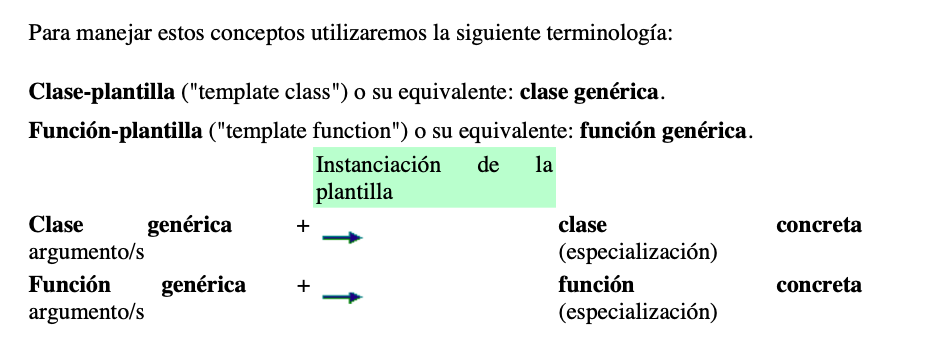
\includegraphics[width=1\linewidth]{Grafica}





    \item Elegir un intervalo de solución
    \item  Elegir un intervalo de solución
\end{itemize}
    

\end{document}